%File: formatting-instruction.tex
\documentclass[letterpaper]{article}
\usepackage{flairs}%aaai
\usepackage{times}
\usepackage{helvet}
\usepackage{courier}
\usepackage{url}
% for figure grid
\usepackage{graphicx}
\graphicspath{ {figures/} }
\usepackage{caption}
\usepackage{subcaption}
\usepackage{wrapfig}
\usepackage{multirow}
\usepackage{tabularx}
\usepackage{paralist}
\usepackage{colortbl}
\usepackage{dingbat, pifont}
\definecolor{Gray}{gray}{0.9}

\usepackage{array} %for table fix width

\frenchspacing
\setlength{\pdfpagewidth}{8.5in}
\setlength{\pdfpageheight}{11in}
\pdfinfo{
/Title (Enhancing Linux Kernel Real-Time Performance through Centralized Timer Interrupt Handling)
/Author (Anonymous)}
\setcounter{secnumdepth}{0}  

\begin{document}
% This file is an adoption of the style file for AAAI Press 
% proceedings, working notes, and technical reports.  This file is made 
% with minimal changes by explicit permission from AAAI.
%
\title{Enhancing Linux Kernel Real-Time Performance through Centralized Timer Interrupt Handling}
\author{
\begin{tabular}{lllll}
  Zhouyi Zhou & Zhili Liu & Shancong Zhang & Jiemin Li & Dengke Du \\
  Mengke Sun  & Zhiqiang Wang & Hongyan Liu & Guoxin Xu & Yexin Han\\
%  & Dengke Du & Mengke Sun  & Zhiqiang Wang & Hongyan Liu & Guoxin Xu & Yexin Han\\
\end{tabular}
\\
Beijing UCAS Space Technology Co Ltd, Beijing, China\\
\{zhouyi.zhou, zhili.liu, sam.zhang, jiemin.li,
dengke.du, mengke.sun, zhiqiangwang, hongyan.liu,
xuguokai, hanyexin\}@ucas.com.cn\\ 
}

\maketitle

\begin{abstract}
In real-time and high-performance computing environments, predictable CPU behavior and low-
latency response are critical. The Linux kernel, by default, distributes periodic timer interrupts
(ticks) across all CPU cores, issues inter-processor interrupts (IPIs) and scheduling disturbances
that hinder deterministic performance. This paper investigates a method for improving Linux
kernel real-time behavior by centralizing timer interrupt handling and inter-processor interrupts
on periodically invoked function. We analyze the mechanism in detail, explain the interplay with
RCU context-tracking, and demonstrate the practical benefits both in a GPIO toggling environment
and a inter-processor communication environment. Our experiments show significant
improvements in interrupt latency and scheduling predictability, enabling more efficient real-time
and user-space networking applications. 
\end{abstract}


\section{Introduction}
Modern high-performance and real-time systems increasingly demand predictable CPU behavior,
low interrupt latency, and minimal system noise. However, general-purpose operating systems
like Linux are not originally designed with these strict requirements in mind. In particular, two key
sources of execution disturbance are periodic timer interrupts and inter-processor interrupts (IPIs)
— each of which independently contributes to unpredictability and jitter in CPU-bound workloads.
Timer Interrupts: The Linux kernel schedules periodic timer interrupts (commonly known as ticks)
on every CPU core to maintain kernel housekeeping, timekeeping, and scheduling. These
interrupts invoke routines for updating system time, triggering task rescheduling, handling timer
expiration, real time process bandwidth control, and advancing internal kernel mechanisms. For
typical workloads, such periodic processing is harmless or even necessary. However, for latency-
sensitive applications — such as user-space network packet processing, real-time control loops,
or audio/video pipelines — these timer interrupts pose significant interference by breaking
deterministic CPU execution.


While mechanisms like NOHZ\_FULL aim to reduce the frequency of such timer ticks, they cannot
completely eliminate them. Even in nohz\_full mode, the tick timer still fire periodically. Thus, strict
real-time applications still face residual interruptions even on nominally “isolated” cores.
Inter-Processor Interrupts (IPIs): In parallel with timer-related disturbances, IPIs represent another
major source of noise. IPIs are used in the kernel to coordinate state changes between cores —
for example, to trigger TLB shootdowns, wake remote tasks, or synchronize RCU grace periods.
From the perspective of an application pinned to a specific core, IPIs are unpredictable and
asynchronous, and can cause unwelcome preemption or context switches.
Although disabling timer interrupts may reduce local noise, it does not automatically prevent a
core from receiving IPIs initiated by other cores or subsystems. This means that even a core
exempt from ticks may still be interrupted arbitrarily due to kernel-wide coordination
mechanisms.


Our Approach: Full Isolation by timer bypass and IPI suppression. In this paper, we present a novel
and more aggressive approach to CPU isolation in Linux: We completely disable timer interrupt
processing on selected cores, ensuring no kernel tick-related activity occurs locally; We suppress
all non-essential inter-processor interrupts to those cores, using targeted kernel patches and
configuration to redirect such coordination elsewhere or delay it entirely. This level of isolation is
not achievable with existing mechanisms like NOHZ\_FULL or isolcpus alone. Our solution explicitly
separates time-related kernel responsibilities and reassigns them to maintenance mechanism,
which periodically execute the timer functionalities required for global correctness. Meanwhile,
isolated cores run continuously without being interrupted by either local timers or remote IPIs.
This approach is particularly effective in scenarios like GPIO toggling, where high precision and
low-latency response are critical, allowing the Linux isolation kernel to efficiently manage interrupts,
isolate processing on specific cores, and ensure that GPIO outputs are triggered in a timely manner,
free from interrupt interference or other system task disruptions.


\section{Related Work}\label{BG} 
\subsection{Timer Interrupt Control in the Linux Kernel}
The timer ticker design for Operating Systems has long exist before Linux kernel was
developed\cite{Corbet}.
The Linux kernel schedules periodic timer interrupts (ticks) on each CPU core for timekeeping,
process accounting, and scheduler activation. These interrupts are typically generated at (250 - 1K) Hz
and cause the kernel to preempt running tasks for internal maintenance.
To reduce this overhead, tickless systems were introduced. The NO\_HZ feature disables timer
interrupts on idle CPUs, and its extension, NOHZ\_FULL, attempts to eliminate ticks even during
user-space execution\cite{KernelDocNOHZ}. However, timer ticks still occur on NO\_HZ/NOHZ\_FULL CPUs because the
kernel want to do statistics works\cite{stackoverflow}.
These mechanisms help reduce timer-induced jitter but do not eliminate all sources of latency.

\subsection{Inter-Processor Interrupts (IPIs) and Their Effects}
Inter-process interrupts (IPIs) in Linux can impact real-time performance by introducing
unpredictable latency, as they force a CPU to handle interrupts from another processor,
potentially preempting time-critical tasks. In real-time systems, where deterministic scheduling
and minimal latency are crucial, IPIs—used for tasks like TLB flushes, cache management, or
scheduler balancing—can cause delays if they trigger during high-priority real-time execution.
Unlike timer interrupts, IPIs are externally triggered and often asynchronous. This means that even
tickless CPUs may receive unexpected IPIs, introducing nondeterministic latency and cache
disruptions. Existing work recognizes this as a major obstacle to achieving strict real-time
performance in Linux \cite{YuxinRen}.


To mitigate the impact of inter-processor interrupts (IPIs) on real-time performance, we must
systematically identify and address each IPI source individually. For instance, unloading block
devices in Linux will trigger IPI, we avoid dynamically unloading them in real-time critical
environments. Similarly, since CPU frequency statistics require a IPI to get frequency from another
CPU, we disable frequency scaling or use a fixed frequency mode to eliminate such overhead. By
analyzing and selectively disabling IPI-inducing operations—such as TLB shootdowns, RCU
callbacks, or scheduler balancing—we eliminate all the unnecessary cross-core interruptions,
ensuring deterministic latency for real-time tasks. This targeted approach, combined with CPU
isolation and IRQ affinity tuning, helps maintain hard real-time guarantees in Linux systems.


\subsection{CPU Isolation Techniques}
The Linux isolcpus and irqaffinity \cite{KernelDocParam} allow a processor core to be isolated from the general
scheduler and external interrupts, effectively preventing it from handling most kernel tasks and
services such as RCU callbacks. However, these mechanisms do not prevent all types of
interruptions. Specifically, they cannot disable timer interrupts or inter-processor interrupts (IPIs),
which may still be delivered to the isolated core. As a result, while these tools can reduce
interference from the operating system, they do not achieve complete isolation at the hardware
interrupt level.


The Redhawk Linux RTOS\cite{redhawk} eliminates the impact of clock interrupts on the OS through its unique
technologies. By modifying mechanisms such as , it significantly reduces the influence of inter-core
interrupts on system performance. However, the system does not completely eliminate inter-core
interrupts on isolated cores; instead, it allows them to occur conditionally.

\section{Methodology}\label{BE}

This section describes the kernel-level design, isolation strategy, and implementation workflow we
employed to eliminate system noise on real-time application cores without delegating
maintenance tasks to external housekeeping cores. In contrast to traditional separation
approaches, our system uses a novel method where the application core periodically invokes
maintenance handlers via a centralized interface. This design is made possible through the custom
Isolator API v0.1, which we developed to enable complete tick and IPI suppression while
preserving system functionality through cooperative execution.


\subsection{System Design Overview}

Our approach is centered on full in-core isolation, where a single CPU core both executes the real-
time workload and explicitly handles minimal kernel maintenance at predefined intervals. Instead
of relying on external housekeeping cores, the application periodically calls into a user-space
handler () that triggers deferred kernel functions such as timekeeping, scheduling updates, and
RCU progress.


To achieve this, we built an isolation runtime system that operates in three main phases:
Start of Isolation: The application invokes with a bitmask specifying which categories of kernel
noise to suppress (e.g., timer ticks, IPIs, and resched interrupts).


Polling Execution Phase: The application enters a tight loop performing real-time operations (e.g.,
GPIO toggling). During each iteration, it calls at regular intervals to perform minimal
kernel duties without relying on interrupts.


End of Isolation: When the application finishes or relinquishes real-time control, it calls to restore
the core’s default interrupt behavior.


This model results in a hybrid kernel-user coordination framework that blends user-driven
maintenance with aggressive in-kernel suppression of interruptions

\begin{figure}
    \centering
    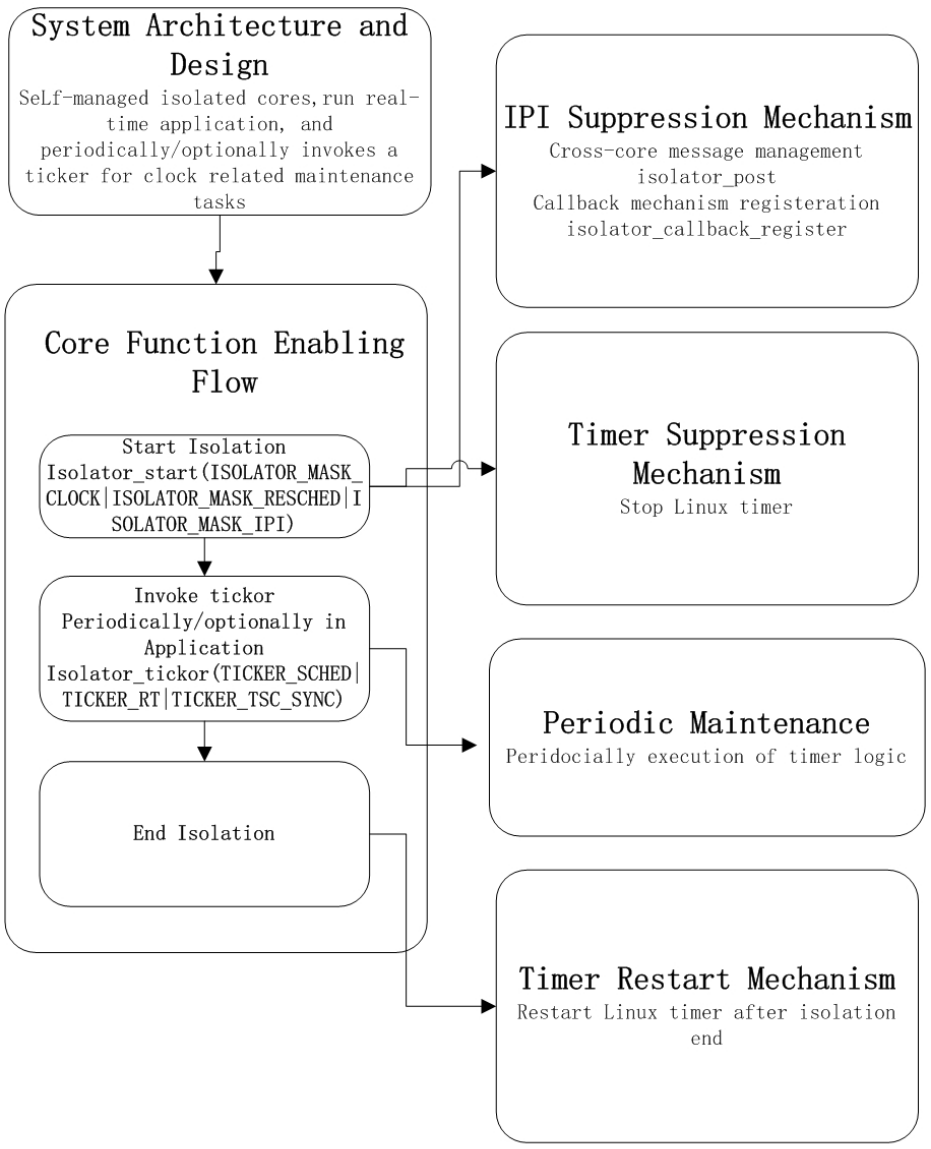
\includegraphics[width=0.85\columnwidth]{architecture.png}
    \caption{System architecture.}
    \label{fig:architecture}
\end{figure}

\subsection{Interrupt Suppression and Timer Bypass} 
The kernel was modified to recognize the isolator state of a core. When isolation is active, the
core's local tick logic (in and ) is bypassed entirely unless triggered by . Furthermore, we suppress
or reroute all asynchronous IPIs that could disrupt the core. This includes:
RCU and TLB IPIs: Deferred and processed only during the maintenance invocation.
Reschedule Interrupts: Suppressed via unless manually enabled.
Frequency Scaling: Disabled to prevent CPU freq gathering triggered IPIs.
To maintain a valid notion of system time, we provide a monotonic time interface (), which returns
a linealized timestamp in microseconds. Additionally, allows predictable wake-ups in polling loops
without enabling standard kernel timers.

\subsection{Memory and Communication Management}
Memory operations required during isolation are supported through and to ensure deterministic
behavior without invoking general-purpose allocators. For core-to-core interactions, provides a
safe messaging mechanism by proxying requests to another non-isolated core. This eliminates the
need for interrupts to wake remote threads.
Callback functions for inter-core communication are registered via to allow non-intrusive
notification delivery. This design ensures that all communication remains strictly user-driven.

\subsection{Isolation Monitoring and Debugging}
To support verification and monitoring, we implemented a real-time statistics collector using ,
which tracks the types and number of interrupts blocked or deferred on each core. These statistics
allow developers to verify the success of isolation policies under different workloads and tuning
configurations.

\subsection{Evaluation Strategy}
Our experimental evaluation used a DPDK-based real-time packet processing workload running on
a custom-patched Linux kernel (v5.15 PREEMPT\_RT). We allocated two isolated cores to handle
high-frequency RX/TX polling. For latency measurement, we replaced hardware timestamping
with GPIO toggling on a Phytium board, captured using an oscilloscope to ensure precise,
external visibility.
We tested the jitter of DPDK forwarding using a packet generator.
For the GPIO measurement, we used a user-space program to toggle a GPIO pin at a fixed
frequency, generating a square wave. The jitter was observed on an oscilloscope by capturing the
edge fluctuations of the signal, which allowed us to assess the timing precision and real-time
stability of the system under different loads.


\section{Implementation Details}
This section presents a detailed overview of the kernel-level modifications we introduced to
support high-determinism, low-jitter execution on isolated CPUs for high-performance, real-time
packet processing. These modifications are implemented within four critical subsystems of the
Linux kernel: RCU (Read-Copy-Update), the Real-Time Scheduler, SMP/IPI handling, and Timer Tick
Management. In addition, we introduce a lightweight per-CPU isolation tracking mechanism that
guides these subsystems to adapt their behavior dynamically based on the isolation state of each
core.

\subsection{Kernel Modifications Overview}
To enable CPU isolation at a fine granularity and ensure minimal OS interference on application-
dedicated cores, we performed targeted changes across the kernel. The key goals are to:
Eliminate unnecessary kernel activity on isolated CPUs,
Avoid inter-processor communication (e.g., IPIs) to reduce latency spikes,
Defer time-based maintenance (e.g., scheduling enforcement) to application-controlled contexts,
Maintain correctness of core kernel mechanisms while enabling custom runtime models.
To coordinate the behavior of different kernel components, we define the following per-CPU data
structure:
\begin{verbatim}
DEFINE_PER_CPU(atomic_t, isolator_counters[CONFIG_NR_CPUS]);
\end{verbatim}
Each entry in this array acts as a flag indicating whether the corresponding CPU is currently under
isolation. This flag is incremented by user-space applications via a custom system call or API
(isolator\_ticker()) and is read by kernel components to selectively disable or defer their operations.


\subsection{RCU Grace Period Handling}
This modification ensures that CPUs marked as isolated are treated as being in a permanent
quiescent state by the RCU subsystem. By doing so, the system avoids unnecessary waiting on
isolated cores during RCU grace periods. This approach maintains forward progress of the RCU
mechanism while eliminating dependencies on cores that are no longer expected to participate in
normal kernel activity.

Such treatment is especially crucial in real-time and low-latency systems where isolated CPUs are
fully dedicated to user-level workloads and should not incur involuntary kernel participation.
We add following following condition to kernel function rcu\_implicit\_dynticks\_qs:
\begin{verbatim}
if (isolator_counters[rdp->cpu].counter) {
   return 1; // Force quiescent state
}
\end{verbatim}
Technical Implications:
Prevents false-positive RCU stall warnings,
maintains system-wide RCU progress without interference from isolated cores,
Ensures correctness without compromising latency isolation.

\subsection{Real-Time Scheduler Deferral}
The changes to the real-time scheduler timer logic allow the suppression of periodic enforcement
checks on isolated CPUs. Instead of allowing kernel timers to preempt execution at arbitrary
intervals, bandwidth enforcement is deferred and delegated to a new handler (), which can be
invoked explicitly by user-space code.
This redesign ensures that real-time constraints are still respected, albeit under application
supervision, thus balancing temporal determinism with system integrity.
We modify the core real-time scheduler timer routine (sched\_rt\_period\_timer) as follows:
\begin{verbatim}
if (__this_cpu_read(ticker_counter) != 0) {
    __this_cpu_write(ticker_rb, rt_b); // Save rt_bandwidth
    __this_cpu_write(ticker_rt_period, rt_b->rt_period);
   return HRTIMER_NORESTART;
}
\end{verbatim}
This suppresses the default timer behavior when the CPU is isolated.
We also introduce a new explicit handler, which can be invoked periodically:
\begin{verbatim}
void ticker_handle_sched_rt_timer() {
    struct rt_bandwidth *rt_b = __this_cpu_read(ticker_rb);
    if (rt_b && time_elapsed_since_last_check()) {
       unsigned int overrun = calculate_overrun(rt_b);
       do_sched_rt_period_timer(rt_b, overrun);
       __this_cpu_write(ticker_jiffies_rt, jiffies);
   }
}
\end{verbatim}
Technical Implications
Minimizes involuntary kernel preemption on isolated CPUs,
Preserves schedulability enforcement via cooperative, user-controlled mechanisms,
Reduces high-resolution timer overhead in performance-critical execution paths.

\subsection{IPI Suppression}
The suppression of inter-processor interrupts (IPIs) to isolated CPUs eliminates one of the major
sources of external interference and cache coherence disruption in multicore systems. By
modifying the logic responsible for IPI target selection, the kernel dynamically filters out isolated
CPUs from cross-core signaling paths.
This ensures that CPUs dedicated to real-time or latency-sensitive processing remain unaffected
by kernel events originating from other cores, thereby improving predictability and scalability.
Technical Implications
Avoids cache line bouncing and contention due to remote invalidations,
Improves temporal isolation between application cores and system housekeeping,
Enhances real-time scheduling fidelity in multi-core environments.

\subsection{Tickless Operation Enforcement}
The enforcement of tickless operation for isolated CPUs is achieved by disabling the kernel's
internal logic for restarting periodic scheduler ticks. Isolated CPUs are instead allowed to operate
independently of the kernel's timekeeping framework unless explicitly re-engaged by user-level
logic.
A fallback function () is provided to perform minimal time accounting when needed, ensuring
correctness of process time tracking while preserving user-space control.
Technical Implications
Enables fully tickless execution on isolated CPUs, reducing kernel-induced jitter,
Eliminates background timer interrupts that may interfere with deterministic workloads,
Facilitates fine-grained control over timekeeping from user space, which is critical in real-time
systems.

\section{Summary}
Collectively, these kernel-level enhancements enable an isolation-aware runtime model optimized
for deterministic, high-performance execution. Each subsystem is modified in a manner that
preserves overall system correctness while respecting the isolation constraints imposed on
specific CPUs. The design offers both temporal isolation and operational autonomy for real-time
workloads, making it highly suitable for use cases such as packet processing, edge computing, and
embedded systems.
It is also important to note that the maintenance-related ticker handlers introduced in our design
(e.g., and ) are optional in practice. In scenarios where the application cannot afford periodic
interruption for such maintenance tasks, these handlers may be deliberately omitted. The primary
consequence of this omission is that certain kernel statistics—such as process time accounting—
will not be accurately recorded or reported. However, in many mission-critical or latency-sensitive
applications, such statistical data is not essential. Similarly, the periodic handling of inter-processor
interrupt (IPI) functionality can also be safely disabled under specific conditions. For example, if
the application running on an isolated core does not access memory regions mapped via , then the
corresponding IPI-based TLB shootdown mechanism may be skipped without compromising
correctness.
\newpage
% \printbibliography 
\bibliographystyle{flairs} 
\bibliography{references.bib}


% \clearpage
\onecolumn
\section*{Appendix}
This section includes additional sample snapshots of malicious videos.
% \begin{figure}[htp]
%     \centering
%     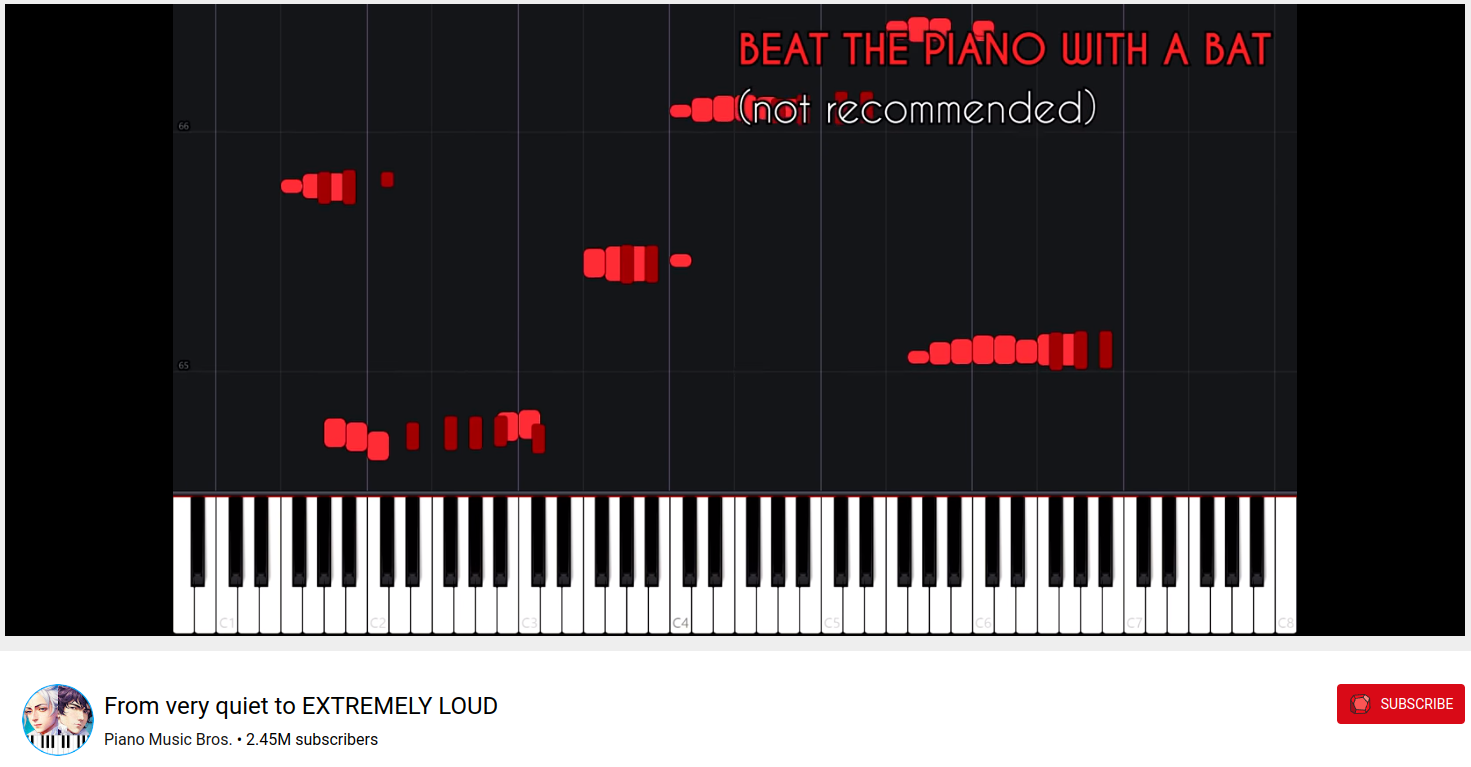
\includegraphics[width=0.6\columnwidth]{figures/malicious_audio.png}
%     \caption{A sample video which includes fast and loud piano notes. Usually in such videos, there is high tempo, no rhythm and varying pitches. The video also includes bright and striking hues, and also suggests a violent action of "hitting the piano with a bat"!}
%     \label{fig:ytkpiano}
% \end{figure}




\begin{figure}[!htb]
  \centering

  \begin{subfigure}{0.45\textwidth}
    \centering
    
\includegraphics[width=\textwidth]{figures/malicious7.png}
    \caption{}
    \label{fig:image_a}
  \end{subfigure}
  \hfill
  \begin{subfigure}{0.45\textwidth}
    \centering
    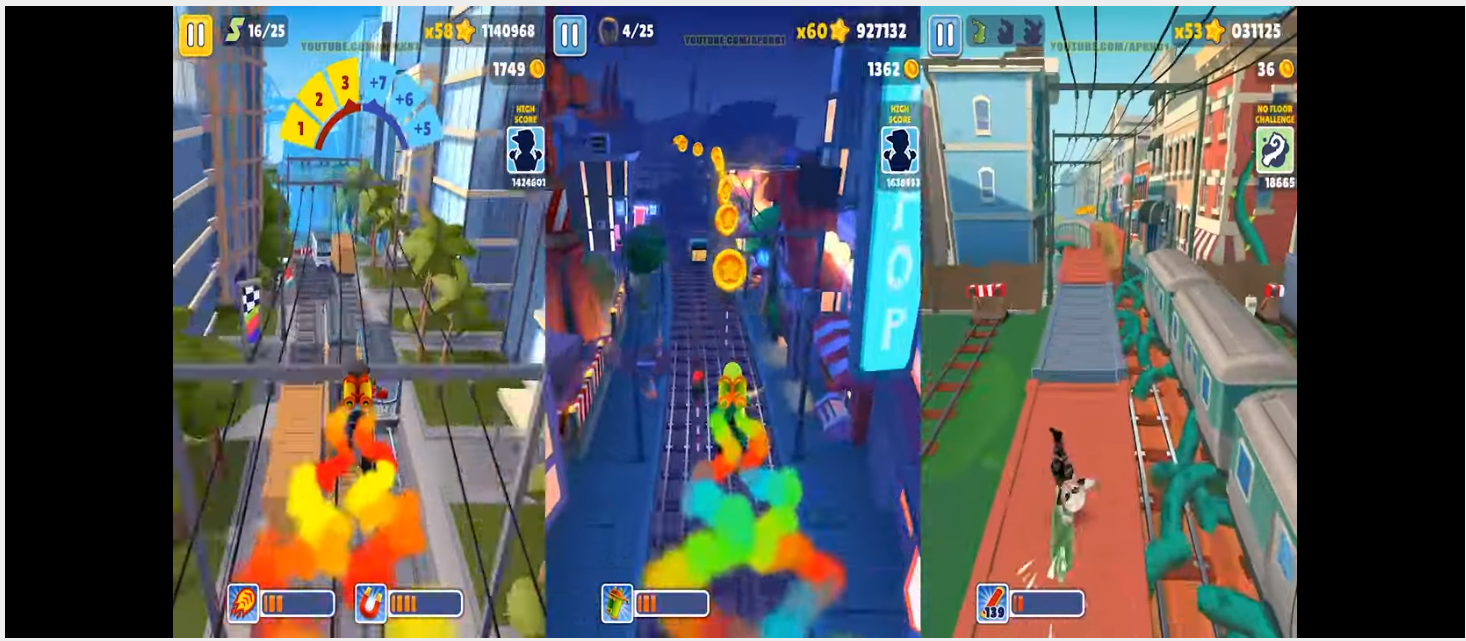
\includegraphics[width=\textwidth]{figures/malicious8.png}
    \caption{}
    \label{fig:image_b}
  \end{subfigure}

  \caption{a) shows a gameplay having striking colors which includes 2 different animations in 2 halves of the screen. b) shows a sample gameplay video for the Subway Surfer game displayed in a split-screen layout.}
  \label{fig:group_of_images}
\end{figure}

\begin{figure}[!htb]
  \centering

  \begin{subfigure}{0.45\textwidth}
    \centering
    
\includegraphics[width=0.8\textwidth]{figures/malicious5.png}
    \caption{}
    \label{fig:image_disgust}
  \end{subfigure}
  \hfill
  \begin{subfigure}{0.45\textwidth}
    \centering
    
\includegraphics[width=\textwidth]{figures/malicious9.png}
    \caption{}
    \label{fig:image_angry}
  \end{subfigure}

  \caption{a) shows a disgusting and scary character b) shows a furious and frightening PacMan.}
  \label{fig:disgusting}
\end{figure}

\begin{figure*}[!h]
    \centering
    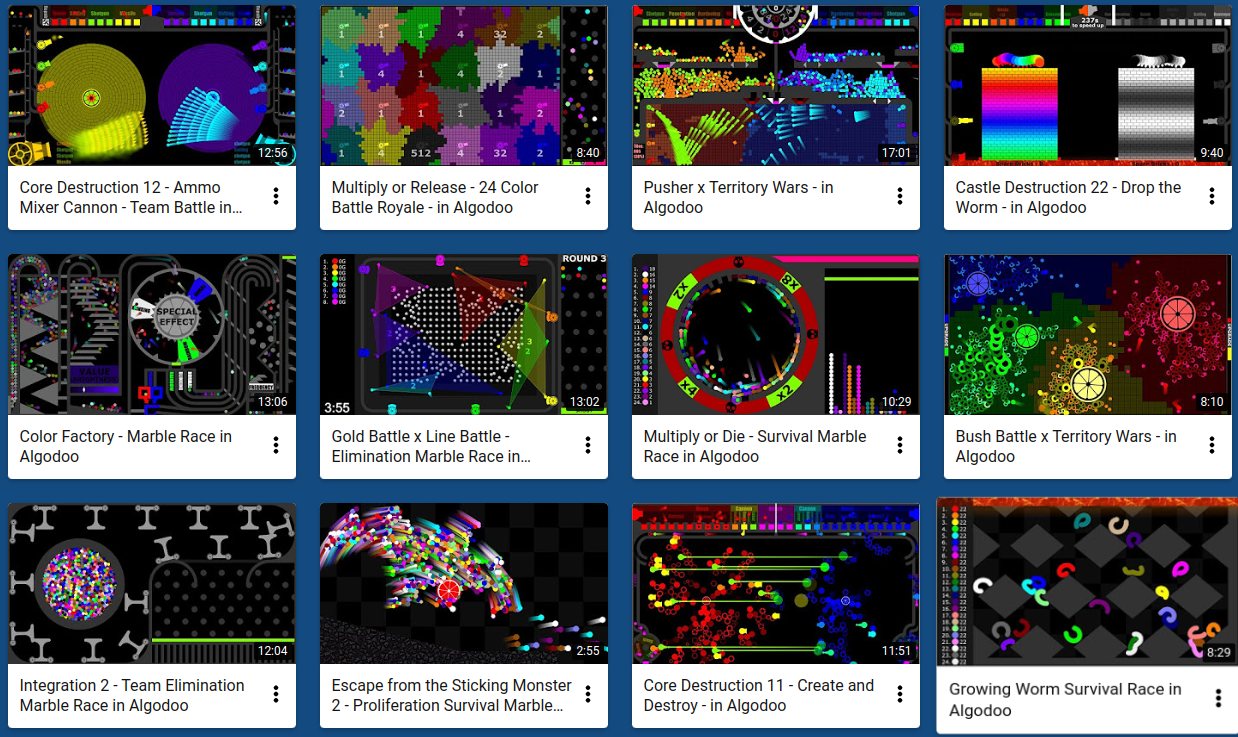
\includegraphics[width=0.8\textwidth]{figures/maliciou3.png}
    \caption{Videos of animations on YouTube Kids which include tiny fast-moving objects with bright colors.  The music soundtrack includes heavy metal and rock music.}  
    \label{fig:model}
\end{figure*}


% \begingroup
% \renewcommand{\arraystretch}{1.6}
% \begin{table}[h]
% \centering
% \begin{tabularx}{0.45\textwidth} { 
%   >{\raggedright\arraybackslash}X 
%   | >{\centering\arraybackslash}X 
%   | >{\centering\arraybackslash}X 
%   | >{\centering\arraybackslash}X
%   | >{\centering\arraybackslash}X 
%   | >{\centering\arraybackslash}X}
 
%  \textbf{Model} & \textbf{Layers} & \textbf{Patch Size} & \textbf{MLP Dim} & \textbf{Heads} & \textbf{Param} \\
%  \hline
%  \hline
%  ViT-B/16 & 12 & 16 & 3072 & 12 & 86M\\
%  ViT-B/32 & 12 & 32 & 3072 & 12 & 86M\\
%  % ViT-L/14 & 24 & 1024 & 4096 & 16 & 307M\\
% \end{tabularx}
% \caption{Comparison of CLIP base models.}
% \label{table:modelcomp}
% \end{table}
% \endgroup

\end{document}
